% 개념 59 152-28(본책 152쪽) — 왼쪽 A, 오른쪽 위 B, 오른쪽 아래 C·D 로 나뉜 직사각형 색칠 영역도. 스캔 그림을 TikZ 로 다시 그림.
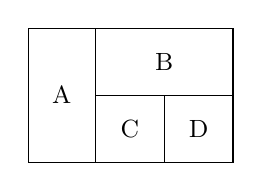
\begin{tikzpicture}[line width=0.5pt, font=\small]
  \draw (0,0) rectangle (2.6,1.7);
  \draw (0.85,0) -- (0.85,1.7);
  \draw (0.85,0.85) -- (2.6,0.85);
  \draw (1.725,0) -- (1.725,0.85);
  \node at (0.425,0.85) {$\mathrm{A}$};
  \node at (1.725,1.275) {$\mathrm{B}$};
  \node at (1.2875,0.425) {$\mathrm{C}$};
  \node at (2.1625,0.425) {$\mathrm{D}$};
\end{tikzpicture}
